\documentclass[tikz,border=3pt]{standalone}
\usepackage{pgfplots}
\pgfplotsset{compat=1.18}
\usetikzlibrary{arrows.meta,positioning,calc}
\begin{document}

\hyphenpenalty=10000\exhyphenpenalty=10000
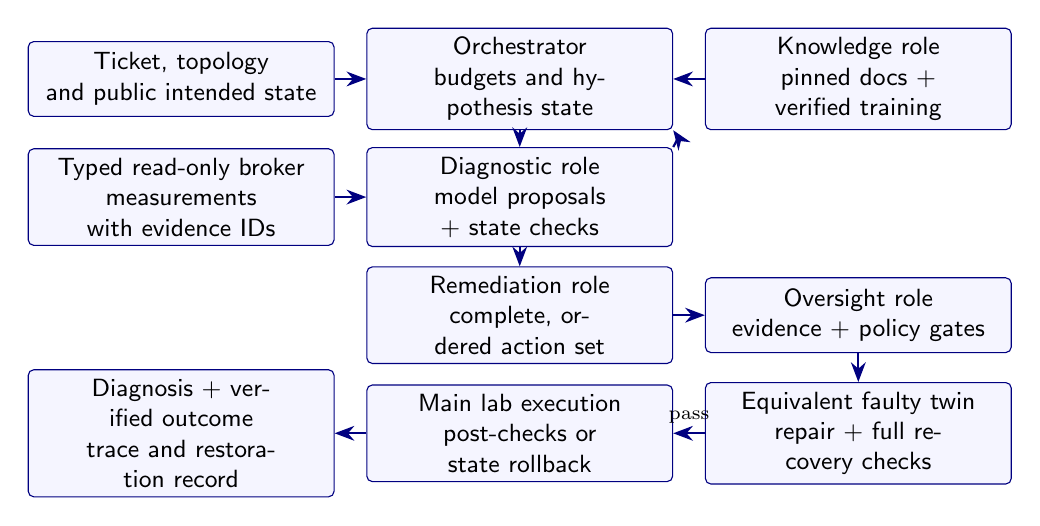
\begin{tikzpicture}[font=\sffamily\small,box/.style={draw=blue!50!black,fill=blue!4,rounded corners=2pt,align=center,minimum height=0.95cm,text width=3.65cm},arr/.style={-{Stealth[length=2.5mm]},thick,draw=blue!50!black}]
\node[box] (in) at (0,0) {Ticket, topology\\and public intended state};
\node[box] (orch) at (4.3,0) {Orchestrator\\budgets and hypothesis state};
\node[box] (know) at (8.6,0) {Knowledge role\\pinned docs + verified training};
\node[box] (diag) at (4.3,-1.5) {Diagnostic role\\model proposals + state checks};
\node[box] (broker) at (0,-1.5) {Typed read-only broker\\measurements with evidence IDs};
\node[box] (repair) at (4.3,-3.0) {Remediation role\\complete, ordered action set};
\node[box] (over) at (8.6,-3.0) {Oversight role\\evidence + policy gates};
\node[box] (twin) at (8.6,-4.5) {Equivalent faulty twin\\repair + full recovery checks};
\node[box] (main) at (4.3,-4.5) {Main lab execution\\post-checks or state rollback};
\node[box] (out) at (0,-4.5) {Diagnosis + verified outcome\\trace and restoration record};
\draw[arr] (in)--(orch);\draw[arr] (know)--(orch);\draw[arr] (orch)--(diag);
\draw[arr] (broker)--(diag);\draw[arr] (diag)--(repair);\draw[arr] (repair)--(over);
\draw[arr] (over)--(twin);\draw[arr] (twin)--node[above,font=\scriptsize]{pass}(main);\draw[arr] (main)--(out);
\draw[arr,dashed] (diag.north east) to[bend right=35] (orch.south east);


\end{tikzpicture}\end{document}
